\chapter{Introduction} \label{chap:intro}
%   talk about self-reported pain and intensity estimation
%   why didn't I do any intensity estimation stuff?
%   Regression is difficult??? Classification is a different thing.
%   take about the fact that you are doing one frame and a time and
%   other methods might be better because they can do sequences.

  The human face is one of the most researched objects in image analysis
  and computer vision \cite{S.ZafeiriouA.PapaioannouI.KotsiaM.A.Nicolaou}.
  It has wide ranging applications from Human
  Computer Interaction (expression recognition) to law enforcement (face recognition).
  Its study necessitates the development of a wide range of machine
  learning and computer vision research.

  Facial Action Unit detection \cite{Corneanu2016} is chosen in this work due
  to it's popularity and available benchmarks.
  The Facial Action Coding System (FACS) developed by Ekman and Friesen,
  provides a systematic way to study any kind of facial expression,
  by representing them as a combination of individual facial muscle actions
  known as Action Units (AU). Automating the process of detecting AUs is difficult
  because they have non-linear interactions \cite{S.EleftheriadisO.Rudovic}
  and often occur in very low intensities.

  Deep learning is emerging as a powerful tool in modelling a wide range of patterns
  in data, it has been applied to the problem of detecting AUs a number of times and achieved
  good classification scores \cite{Khorrami2015,Jaiswal2016,Kim2016,Gudi2015,Ghosh2015}.

  There exist many datasets containing images and videos of faces and it is a general
  observation that unlabelled datasets are far more abundant than labelled ones.
  In particular for AUs because manual AU
  annotation is laborious and requires trained expert coders.
  Datasets containing AUs have a few key differences to datasets typically used with
  deep networks, these are:
  \begin{enumerate}
    \item The variation between images is lower than the datasets typically used
    to train deep neural networks because AUs can be signified by subtle changes.
    \item They contain fewer images, for example compared to ImageNet\cite{Deng2009} which has 3.2 million labelled images.
    \item The possibility for AUs to occur simultaneously
    \item Non-uniform AU occurrence frequencies as many frames in a video may
    contain no AU occurrences (neutral faces) and some AUs may occur a lot less or a lot more than others.
  \end{enumerate}

  This project aims to tackle these issues by employing the use of autoencoders,
  which are neural networks whose objective is to reproduce their input.
  These are often used to pretrain the weights of classifying networks \cite{googlepretrain}.
  This process of pretraining is generalised so that it can be performed simultaneously with
  the classification training step. This results in a single cost function, which changes during training.
  The idea being that this joint training
  encourages the autoencoder to learn useful features. Furthermore a variety of preprocessing methods such as mean face subtraction and contrast normalisation
  are tested to see which give the best classification results and work best with the joint
  autoencoder and classifier training. These experiments are carried out in a constrained setting
  where even very low intensity AUs are treated as positive examples and the training set is not artificially expanded.

  \begin{figure}
   \centering
   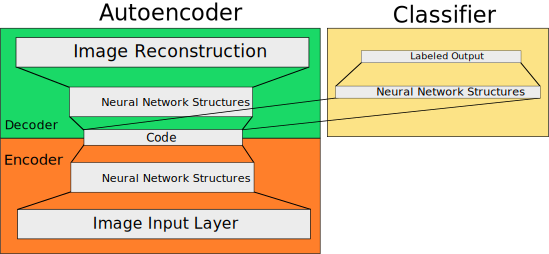
\includegraphics[width=0.8\textwidth]{illustrations/simple_network.pdf}
   \captionof{figure}{General structure of the proposed network. Each rectangle
   represents many layers of neurons and the thin lines represent connections between layers.
   This diagram serves as a very high level description of the structure this project will
   investigate, the boxes in the hidden layers, called neural network structures may contain
   a variety of components including convolutional layers, fully connected layers, dropout layers
   and so on.}
  \end{figure}

  \section{Contributions}
    This work proposes a novel network structure for joint autoencoder and classifier training and tests it with
    the following methods:
    \begin{itemize}
      \item A set of pre-processing methods, such as mean face subtraction and contrast normalisation.

      \item A variety of convolutional architectures and a fully connected networks.

      \item A balancing function, referred to as the alpha function, is introduced which evolves during
            training to balance the autoencoder and classifier losses.

      \item Regularisation techinques including Dropout\cite{Srivastava2014} and L2 Regularisation\cite{Ng2004} which aim to improve the chances
            of creating a simpler but more general model and hence reducing over fitting.

      \item Local Contrast Normalisation\cite{Krizhevsky2012} which is a technique that has been shown to improve classification performance in convolutional networks.

      \item The use of Binary Softmax Layers to jointly classify AU occurrences.

    \end{itemize}
    % This paragraph could be a bit more detailed. You contribute:
    % - proposition of a of a novel network structure for joint autoencoder and classifier training
    % - evaluation of different pre-processing methods, transfer functions, network structures, etc. (provide a detailed list)
    % To the end!
    % No substantial performance improvement is noted but interesting dynamics are observed.

    \section{Potential Applications}
      The ability for a computer vision system to accurately classify actions in a
      human face could have a multitude of application. Human computer interfaces (HCI)
      could benefit from a higher bandwidth interactions between computers and humans, adding
      an extra channel to the typical keyboard and mouse. The medical profession would benefit
      as the ability to quantify psychological symptoms using facial expressions might lead to
      quicker diagnoses of illness and more personalised care.

  \section{Thesis Outline}
    \begin{itemize}
      \item {\bf Chapter 2} first reviews the literature regarding AU databases. It then introduces the
            required theory to constructing and evaluating a deep learning model. Lastly it
            reviews literature which uses deep learning to classify AUs.
      \item {\bf Chapter 3} describes the code that was produced to facilitate experimenting with
            the concepts in Chapter 2 and to enact the goals of Chapter 1
      \item {\bf Chapter 4} describes some proposed preprocessing techinques, such as mean face
            and contrast normalisation.
      \item {\bf Chapter 5} detials the models that were evaluated in this project.
      \item {\bf Chapter 6} evaluates the models from Chapter 5 quantitatively and qualitiatively.
      \item {\bf Chapter 7} discusses the whole project,evaluating the stratergies persued and
            proposing future directions.
      \item {\bf Chapter 8} states the conclusions of the project.
  \end{itemize}
